% analysis.tex
%

%% ==============
\chapter{Analysis}
\label{ch:Analysis}
%% ==============
  Using data obtained by the muon modules and the detector as well as other subsystems' data, the muon induced background rates and both spatial and energy distribution can be obtained. Before actual measurements, the modules had to be set up and calibrated. Comparable rates for all modules and 

  %% ===========================
  \section{Gain-, Threshold and Acceleration Voltage Settings}
  \label{ch:Analysis:sec:GainsThresholdsAccVoltages}
  %% ===========================  
  
  A first amplification - linear with acceleration voltage - of the scintillation photons occurs in the photomultiplier tubes. As signals at first seemed too high for the DAQ to handle at nominal values of the datasheet, these were reduced to around \SI{1200}{\volt}. Now, the software gains and thresholds in the ORCA software needed to be set carefully to make 
  
  
  %% ===========================
  \section{Finding the best filter settings}
  \label{ch:Analysis:sec:Finding the best filter settings}
  %% ===========================  
  As the PMT tubes are directly, without any preamplifiers, connected to the DAQ, the signal lengths arriving at the latter are in the order of \SI{20}{\nano\second}. This poses a problem for filters as the sampling rates need to be high and anti-aliasing is inevitable. To find the best settings, a pulser has been set up to create events at known frequency and peak heigth. The signal form \todo{what form} was chosen as closely to the actual shape as possible
 
  \begin{figure}
	\caption{Pulser shape compared to actual signal shape}
  	
\includegraphics[width = 0.9\textwidth]{graphics/dummy.eps}
  \end{figure}
  
  Now, to evaluate filter goodness, the width of the resulting energy histogram, which should, assuming perfect pulser signals and perfect filters, be monoenergetic, was analysed for each filter setting. This resulted in the following set of data:
  
  \begin{table}
	\caption{Energy resolution at different filter settings}
	\centering
	standard filter
	\begin{tabular}{c}
	\SI{50}{\nano\second} gap, \SI{0}{\second} shaping time\\
	
  	\begin{tabular}{ccc}
  		1& 2& 3\\
  		1& 2& 3\\
  		1& 2& 3\\
  		1& 2& 3\\
  	\end{tabular}
  	\end{tabular}\\
  	boxcar filter
  	\begin{tabular}{ccc}
  		1& 2& 3\\
  		1& 2& 3\\
  		1& 2& 3\\
  		1& 2& 3\\
  	\end{tabular}

  \end{table}
  On average, the boxcar filter at shaping lengths \todo{was it shaping?} of \SI{150}{\nano\second} shows the most promising results. This concurs with the settings chosen for the active fpd veto; here slightly longer (around \SI{30}{\nano\second}) but comparable signals occur, showing best results at the same filter settings\cite{KevinWierman}.
  
  %% ===========================
  \section{Modules in high magnetic fields}
  \label{ch:Analysis:sec:Modules in high magnetic fields}
  %% ===========================  
  
  %% ===========================
  \section{Module Stability}
  \label{ch:Analysis:sec:Module Stability}
  %% ===========================  
  If consistent  on muon induced background is to be made, the modules need to work stable over the course of days, as rates are supposed to be comparable. For this reason, over the Christmas time 2012, a two weekly measurement has been taken. The timeslot was chosen for the lowly frequented spectrometer hall to exclude outer \todo{D: einfluesse}. For analysis, a simple program to count events in variable time bins was written, creating a rate histogram for all the runs in the measurement period. The following fluctuation could be observed:
  \begin{figure}
	\centering
  	
\includegraphics[width = 0.9 \textwidth]{graphics/dummy.eps}
  \end{figure}
  These are closely related to the fluctuations in atmospheric density, pressure and temperature. If one looks at the data from \todo{find weather station data, see if it fits fluctuations}\todo{maybe cascade data to back it up?}

  %% ===========================
  \section{Module Efficiency}
  \label{ch:Analysis:sec:Module Efficiency}
  %% ===========================  
  The runs used for stability measurements, as well as any other including modules six, seven and eight, can be used to check muon module seven for efficiency. For every other module, the geometry would need to be changed so that the one to be checked is in between at least two other modules.
  For analysis, the function determineEfficiency() \ref{ch:Analysis software:sec:methods of the class run:subsec:determineEfficiency}
  has been written.
  It shows that during the measurement period end of 2012, the efficiencies were at \todo{rerun} \SI{94 }{\percent} which is less than one would expect at a thickness of \SI{5}{\centi\meter}.
  For that reason, the filter settings were checked and changed to the boxcar filter with a gap of 150 ns from the before used \todo{exact name} filter. This lead to an increase in efficiency of about \todo{x percent}.
  As the efficiency is still below expected values, a possible improvement would be to use preamplifiers before signals arrive at the DAQ, which would then need to have a higher sampling frequency and widen the signal timewise.
  
  %% ===========================
  \section{Photo Multiplier Tube Test with $^{60}$Co source} %$\bf{^{60}Co}$
  \label{ch:Analysis:sec:PhotoMultiplierTests}
  %% ===========================
  
  With sets of four photomultiplier tubes being read out over one cable, and, consequently, via one channel, the test of individual PMTs is not trivial. Nevertheless, a method using a \SI{}{\mega\becquerel} $\rm ^{60}Co$ source to trigger events was used to check functionality. Of course, all tubes were able to see the source at any position but rates were expected to rise as the distance to any of the tubes shrank. A source holder was constructed from acrylic glass to shield the user from radiation and to attach the source to the modules, as a large dependence of rate on the position was found when the source was simply duct taped to the modules. As the foil mantling the modules absorbs a non negligible part of the radiation emitted from the source, it had to be ensured that the number of layers was equal for all measurements. This was given only below the modules as the foil has been folded around them at the ends in a gift wrapping way. Thus, the source was pretty far away from the photomultiplier tubes making it more difficult to distinguish between them. A first measurement was then to check for exactly that distinguishability.\todo{insert measurement for small steps over PMTs positions}.
  As one can see a rise in rate at the positions the tubes are located at, it was decided that four measurements per module and side were sufficient, especially as all measurements can afterwards be compared to each other.
  The tube positions at \todo{n,n,n,n cm} were used as measurement positions as well. For each side, a run has been taken containing five minute subruns for every position. Figure \ref{fig:CoRatesPMT} shows the result of these measurements. One can see that the gerneral shape of each side compares very well to the others. Exceptions are \todo{which ones different?}showing slight, but acceptable deviations off the norm.
  \begin{figure}
	\label{fig:CoRatesPMT}
	
  	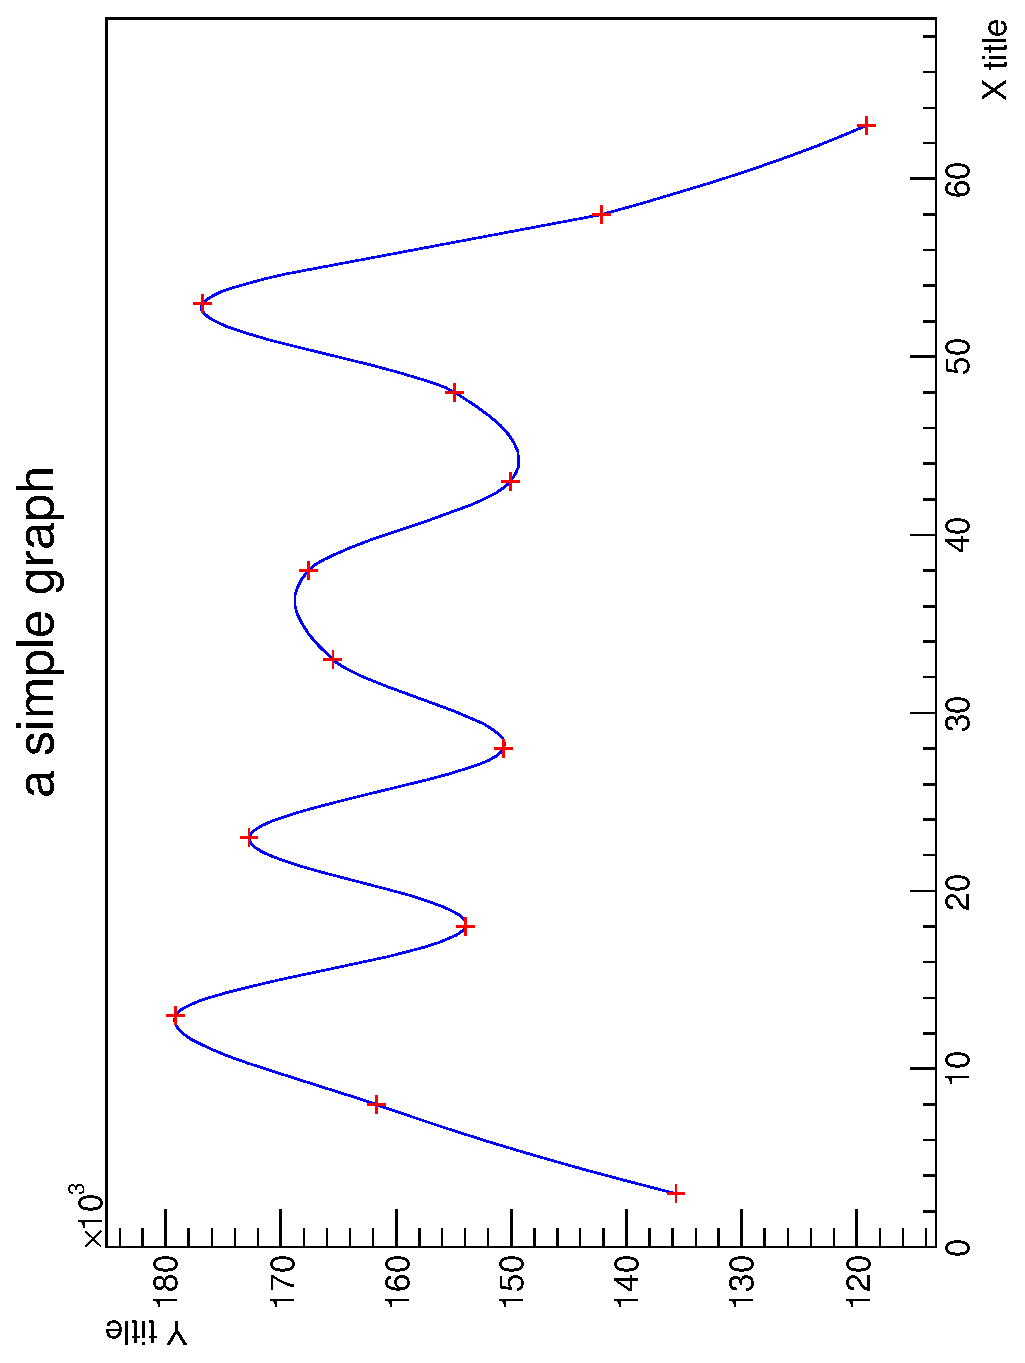
\includegraphics[angle = -90, width = 0.9 \textwidth]{graphics/cobalt/876_parallel_good.eps}
  \end{figure}

  
  %% ===========================
  \section{Coincidence Search between Muon- and Detector Events}
  \label{ch:Analysis:sec:Monitor Spectrometer Measurements}
  %% ===========================  
  If one wants to actually detect background induced by myonic events registered by the muon modules, those events need to be correlated to detector events timewise. For this purpose, the analysis code's class run was extended by the member functions TOFHist()\ref{ch:Analysis software:sec:methods of the class run:subsec:TOFHist()} and TOFMuonDet()\ref{ch:Analysis software:sec:methods of the class run:subsec:TOFMuonDet()}, where the former is used for monitor spectrometer analysis and the latter for the main spectrometer. 
  
  %% =========================
  \subsection{Monitor Spectrometer}
  \label{ch:Analysis:sec:Monitor Spectrometer Measurements:subsec:Monitor Spectrometer}
  %% =========================
  
  Measurements at the monitor spectrometer are easily managable due to the fast accessibility of all the components and the collection of data in a single run file through the mini crate.
  Several hourly runs have been taken under different magnetic field compositions. Both asymmetric magnetic \todo{ref to figure of field lines} and non-axially-symmetric field configurations have been investigated. The TOFHist\ref{ch:Analysis software:sec:methods of the class run:subsec:TOFHist()} function has been used to analyse the data. In all of the settings, a clear peak is visible at around \SI{7}{\micro\second}. As for count rates, they are a lot higher in the asymmetric magnetic field setup as secondary electrons are guided from their point of origin to the detector instead of mostly being magnetically shielded. In this setup, only the reflection through the rise in magnetic field takes its toll on the rate.
  
  \begin{figure}
  	
\includegraphics{graphics/dummy.eps}
  \end{figure}

  %% =========================
  \subsection{Main Spectrometer}
  \label{ch:Analysis:sec:Monitor Spectrometer Measurements:subsec:Main Spectrometer}
  %% =========================
  
  Monitor spectrometer results suggested that the time of flight was well measurable, even if on bigger scale, at the main spectrometer. So, during first light measurements, already during measurement M1, sone runs with asymmetric magnetic field have been taken with switched polarity or turned off pre spectrometer magnets compared to standard setup.
  The data was analysed for each single ring of the FPD, though remains inconclusive at the moment. This might be due to the combbination of muon module position and the magnetic field setup as the wall area covered by the flux tubes and the volume surveilled by the muon modules did not overlap very much.
  
  \begin{figure}
  	
\includegraphics[width = 0.9 \textwidth]{graphics/dummy.eps}
  \end{figure}
  
  Following that presumption, for M6 measurements, the setup was changed. The fluxtube was widened for its outer parts to hit the spectrometer wall in regions around combs n and n \todo{which combs}. This raises the probability of the muons inducing secondary electrons being detected by the modules as well. The resulting flux tube is shown in figure \ref{fig:newFluxTube}. 
  \todo{flux tube including modules for horizontal and vertical view}
  \begin{figure}
	\label{fig:newFluxTube}
	\caption{new flux tube}
  	
\includegraphics[width = 0.9 \textwidth]{graphics/dummy.eps}
  \end{figure}
  \todo{If data will be taken add to analysis.}
  
